
\section{Einrichtung des Debuggers}
In diesem Kapitel wird im Stil eines Tutorials vorgestellt, wie wir vorgegangen sind, um den Debugger zum Laufen zu bekommen. Als Betriebssystem kam Debian zum Einsatz.
\subsection{st-flash Installation und UDEV-Rules}
st-flash wurde von uns anfangs benutzt, um die erzeugten Kompilate auf die Zielplattform zu überführen. In der Installationsroutine ist auch die Installation der wichtigen UDEV-Rules enthalten. Diese werden später noch benötigt.
Zuallererst muss das git-Repository heruntergeladen werden. Zusätzlich, falls nicht vorhanden noch ein paar nötige Build-Tools.
\begin{lstlisting}[language=sh]
sudo apt-get install cmake
sudo apt-get install libusb-1.0-0-dev git
git clone https://github.com/texane/stlink stlink.git
cd stlink.git
\end{lstlisting}
Sobald das Repository heruntergeladen ist, wechseln wir in das Projektverzeichnis und führen die Installationsprozedur aus. Zuerst das "make" und danach kopieren wird die ausführbaren Binarys in das "/usr/bin"-Verzeichnis.
\begin{lstlisting}[language=sh]
make
sudo cp build/Release/st-* /usr/bin
exit # -> Bash neu starten
\end{lstlisting}
Zum Schluss werden die udev-Rules gesetzt, damit das Gerät, also das Target richtig erkannt wird.
\begin{lstlisting}
cd ~/stlink.git
ls -LR | grep rule
cd etc/udev/rules.d
sudo cp *.rules /etc/udev/rules.d
sudo udevadm --reload
sudo udevadm trigger
\end{lstlisting}
\subsection{Download Eclipse}
Um den Debugger zum Laufen zu bekommen, benötigt man zuallererst eine funktionierende Eclipse IDE. Für unser Projekt haben wir uns für 'Eclipse IDE for C/C++ Developers' entschieden erhältlich auf \url{http://www.eclipse.org/downloads/}.
Nach dem Download muss das Paket entpackt werden. In der Kommandozeile funktioniert dies mittel des Befehls 
\begin{lstlisting} 
tar -xzf <eclipse-download-file>
\end{lstlisting}
oder ganz einfach in der grafischen Benutzeroberfläche des Betriebssystems.
Um die Entwicklungsumgebung ausführen zu können, benötigt man Java-Version 1.8 der neuer. 
Die Installation hierfür funktioniert mit den folgenden Commands:
\begin{lstlisting}
sudo su -
echo "deb http://ppa.launchpad.net/webupd8team/java/ubuntu xenial main" | tee /etc/apt/sources.list.d/webupd 8team-java.list
echo "deb-src http://ppa.launchpad.net/webupd8team/java/ubuntu xenial main" | tee -a /etc/apt/sources.list.d/webupd8team-java.list
apt-key adv --keyserver hkp://keyserver.ubuntu.com:80 --recv-keys EEA14886
apt-get update
apt-get install oracle-java8-installer
apt-get install oracle-java8-set-default
exit

\end{lstlisting}
\subsection{Toolchain-Installation}
Um später debuggen zu können, wird ein Kompiler für die Zielplattform benötigt und der spezifische GDB. Diese Tools findet man in Toolchains. Ein Toolchain ist eine komplette Suite, mit Werkzeugen, um für fremde Hardwarearchitekturen Software bauen zu können.
Wir verwenden die GNU-Toolchain. Zunächst laden wir die komplette Toolchain herunter.
\begin{lstlisting}[language=sh]
cd /opt
sudo wget https://launchpad.net/gcc-arm-embedded/5.0/5-2016-q3-update/+download/gcc-arm-none-eabi-5_4-2016q3-20160926-linux.tar.bz2
\end{lstlisting}
Anschließend wird die Datei entpackt.
\begin{lstlisting}[language=sh]
sudo tar -xvjf gcc-arm-none-eabi-4_8-2014q2-20131204-linux.tar.bz2
rm <heruntergeladene Datei>
\end{lstlisting}
Falls die Toolchain-Tools im späteren Entwicklungsprozess im Terminal von überall her gefunden werden sollen, empfielt sich die Anpassung der Datei ~/.bashrc. Dort wird dann einfach die PATH-Variable erweitert.
\begin{lstlisting}[language=sh]
nano ~/.bashrc
# In der Datei zu ergaenzen:
# export PATH=$PATH:/opt/<Name der entpackten tar>/bin
\end{lstlisting}
\subsection{Installieren der Eclipse Toolchain Tools}
In dieser Sektion wird die Installation der Tools innerhalb Eclipse beschrieben.
Zuallererst muss Eclipse geöffnet werden. Die ausführbare Eclipse-Datei befindet sich im entpackten Ordner.
Man wird nach einem Workspace gefragt, einer Arbeitsumgebung. Dies ist der Ordner, in dem Eclipse die Projekte verwaltet. Sofern noch kein Ordner vorhanden ist, einfach einen neuen in Dateisystem erstellen.
Um optimal entwickeln zu können, brauchen wir die ARM GNU Eclipse Toolchain. Um an diese heranzukommen, wählt man zuerst im der oberen Menüleiste im Punkt 'Help' 'Install new Software' aus.
\begin{figure}[h]
\begin{center}
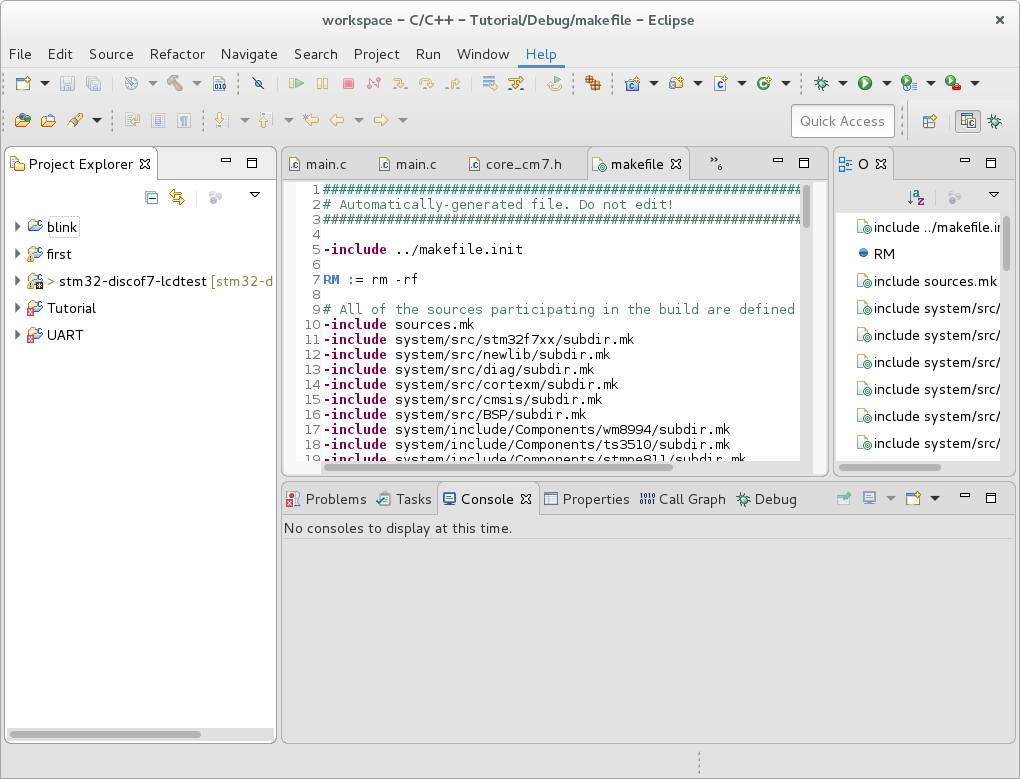
\includegraphics[width=12cm]{grafiken/debugger/EclipseNewSoftware.png}
\label{eclipse_softwareinstallation}
\caption{Eclipse Softwareinstallation}
\end{center}
\end{figure}
Im Fenster 'Install New Software' das Textfeld 'Work with' mit 'GNU ARM Eclipse Plug-ins' füllen. Der richtige Eintrag wird dann vorgeschlagen.
\begin{figure}[h]
\begin{center}
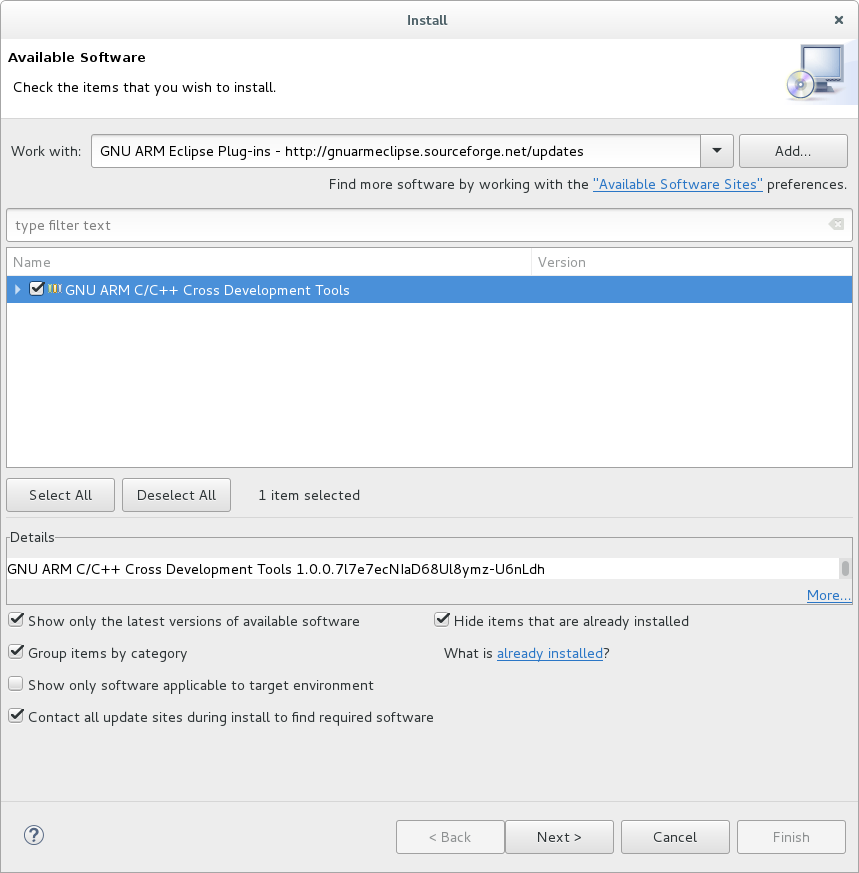
\includegraphics[width=12cm]{grafiken/debugger/GNUauswahl.png}
\label{eclipse_gnu_auswahl}
\caption{Installationsfenster}
\end{center}
\end{figure}
Danach muss der Haken beim Plugin gesetzt werden, ('GNU ARM C/C++ Cross Development Tools') und der Button 'next' betätigt werden. Eventuell muss man jetzt noch ein paar Lizenzverträgen zustimmen. Einfach die Dialoge mit next durchgehen und zum Schluss 'finish' betätigen.
\subsection{Installieren von OpenOCD}
OpenOCD agiert als GDB-Server in unserer Anwendung. Darum müssen wir diese Anwendung noch installieren.
Zuerst muss wieder das GIT-Repository geklont werden. Wir wechseln dazu zum opt-Ordner in unserer Linux-Distribution.
\begin{lstlisting}
cd /opt
# falls noch nicht vorhanden, muss der Ordner gnuarmeclipse erzeugt werden
sudo mkdir gnuarmeclipse
cd gnuarmeclipse
sudo mkdir openocd
cd openocd
sudo git clone http://openocd.zylin.com/p/openocd.git openocd-stm32f7
cd openocd-stm32f7
# zum bauen folgende Befehle verwenden
sudo ./bootstrap
sudo ./configure --enable-stlink
sudo make -j4
# testen, ob alles funktioniert:
cd tcl
../src/openocd -f board/stm32f7discovery.cfg
\end{lstlisting}
Wir arbeiten im /opt-verzeichnis, da das GNU-ARM-Plug-in Konventionen folgt. Wenn man im Ordner gnuarmeclipse Installationen anlegt, werden diese automatisch vom Plug-in erkannt.
Nichtsdestotroz müssen jetzt in Eclipse Einstellungen angepasst werden.
Bei unserer Lösung des Debuggens wird OpenOCD als externes Tool gestartet. Dazu müssen in Eclipse ein Paar Änderungen vorgenommen werden. Unter dem Menüpunkt 'Run'>'External Tools Configurations...' können die Einstellungen hierfür vorgenommen werden.
\begin{figure}[h]
\begin{center}
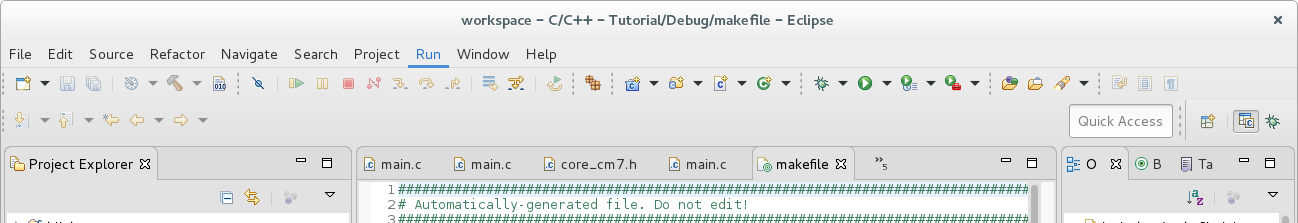
\includegraphics[width=12cm]{grafiken/debugger/RunConfiguration1.png}
\label{eclipse_external_tool_setup}
\caption{Externes Tool einstellen}
\end{center}
\end{figure}
Es müssen dann die Einstellungen wie in \ref{ecplipse_OpenOCD_setting1} vorgenommen werden: 
\begin{figure}[h]
\begin{center}
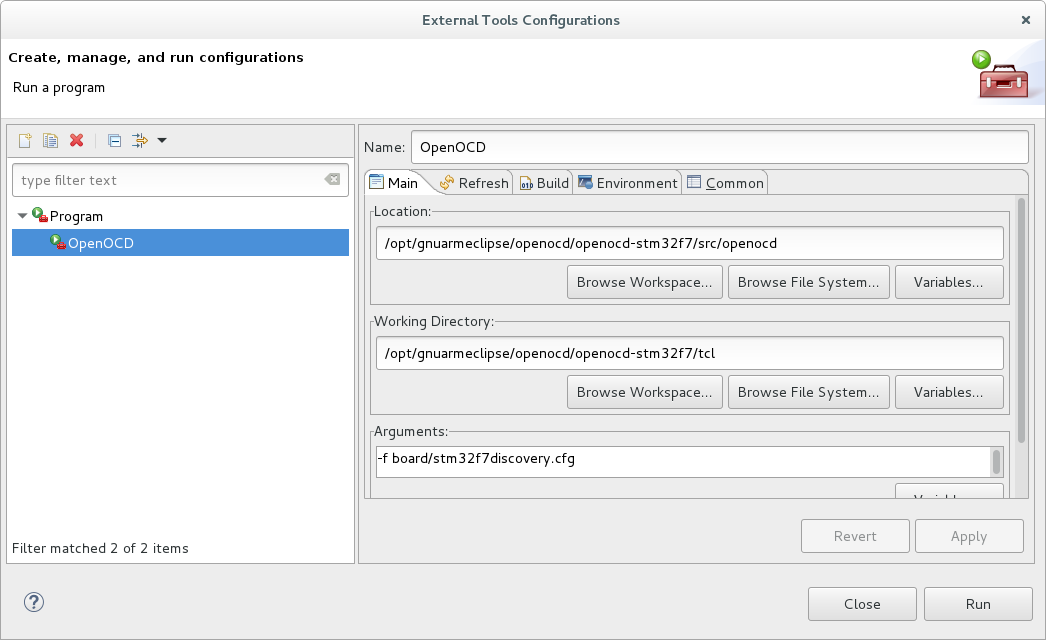
\includegraphics[width=12cm]{grafiken/debugger/OpenOCDsetting.png}
\label{ecplipse_OpenOCD_setting1}
\caption{OpenOCD Settings}
\end{center}
\end{figure}
\newpage
\subsection{GDB-Setup}
In diesem Kapitel wird das Setup des GDB-Debuggings behandelt. Zuvor haben wir die Toolchain für die Entwicklung auf der Zielplattform heruntergeladen. Nun müssen wir nur noch Eclipse beibringen, wie es den GDB aus der Toolchain findet. Außerdem müssen die passenden Parameter zur Ausführung des GDBs gesetzt werden.
Um in die Debug-Einstellungen zu gelangen, muss im Menüpunkt 'Run' 'Debug Configurations... ' gewählt werden. 
\begin{figure}[h]
\begin{center}
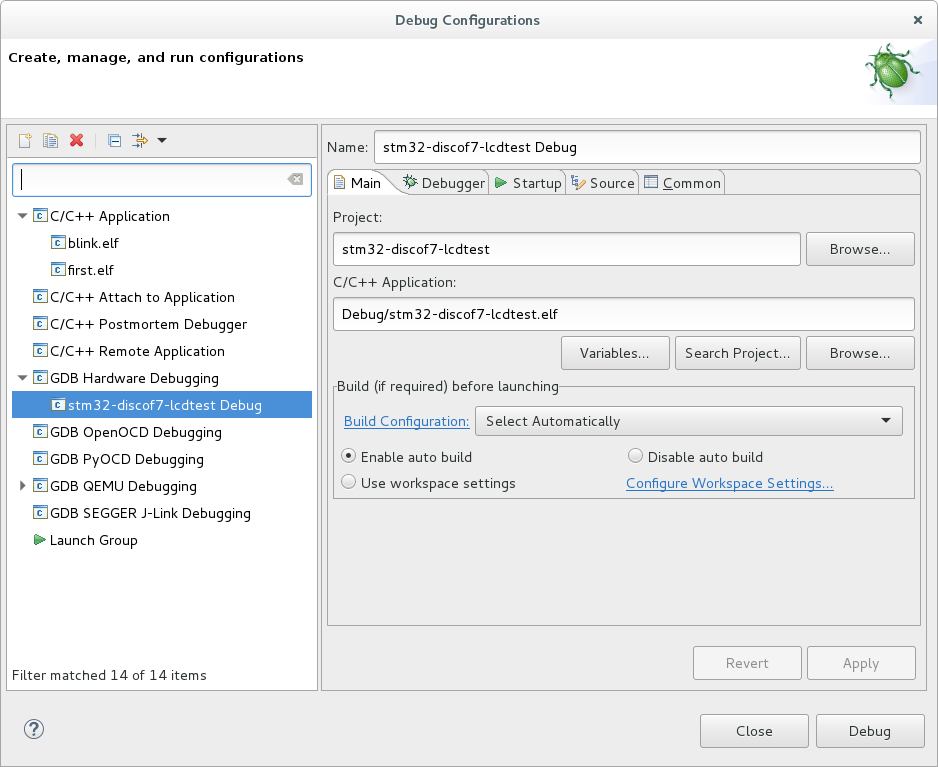
\includegraphics[width=12cm]{grafiken/debugger/GDBsetting1.png}
\label{ecplipse_GDB_setting1}
\caption{GDB Settings}
\end{center}
\end{figure}
Es muss eine neue Konfiguration erzeugt werden, danach werden die Parameter eingetragen. Im Feld Projekt muss der Projektname eingetragen werden, im Feld 'C/C++-Application' der Name des Kompilats.
\begin{figure}[h]
\begin{center}
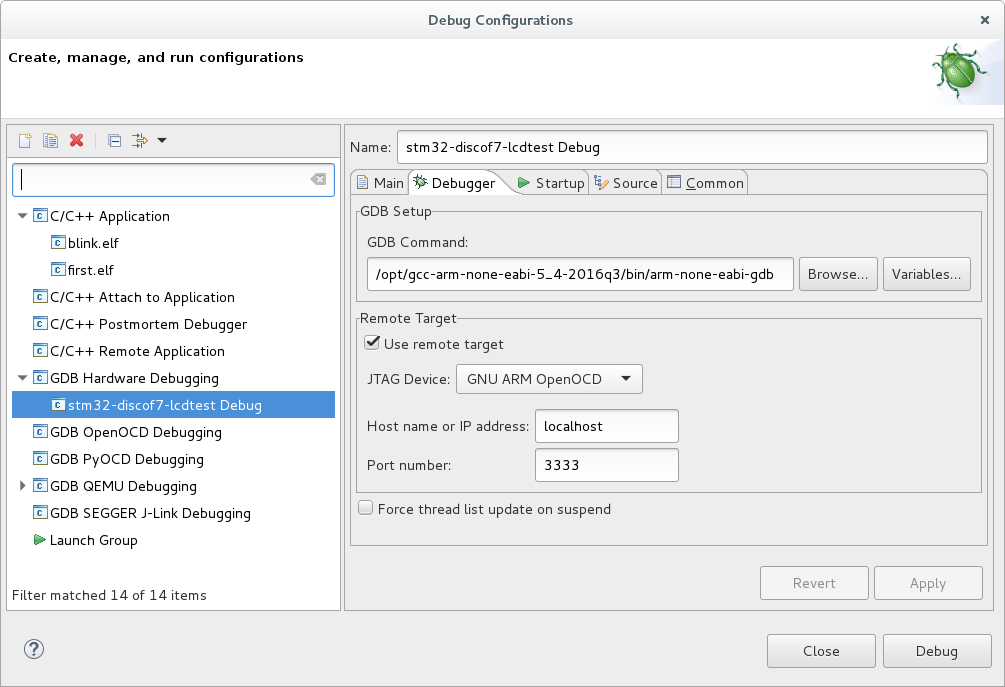
\includegraphics[width=12cm]{grafiken/debugger/GDBsetting2.png}
\label{ecplipse_GDB_setting2}
\caption{GDB Settings 'Debugger'}
\end{center}
\end{figure}
Im Abschnitt 'Debugger' sollte die Konfiguration so aussehen wie in \ref{ecplipse_GDB_setting2}.
\begin{figure}[h]
\begin{center}
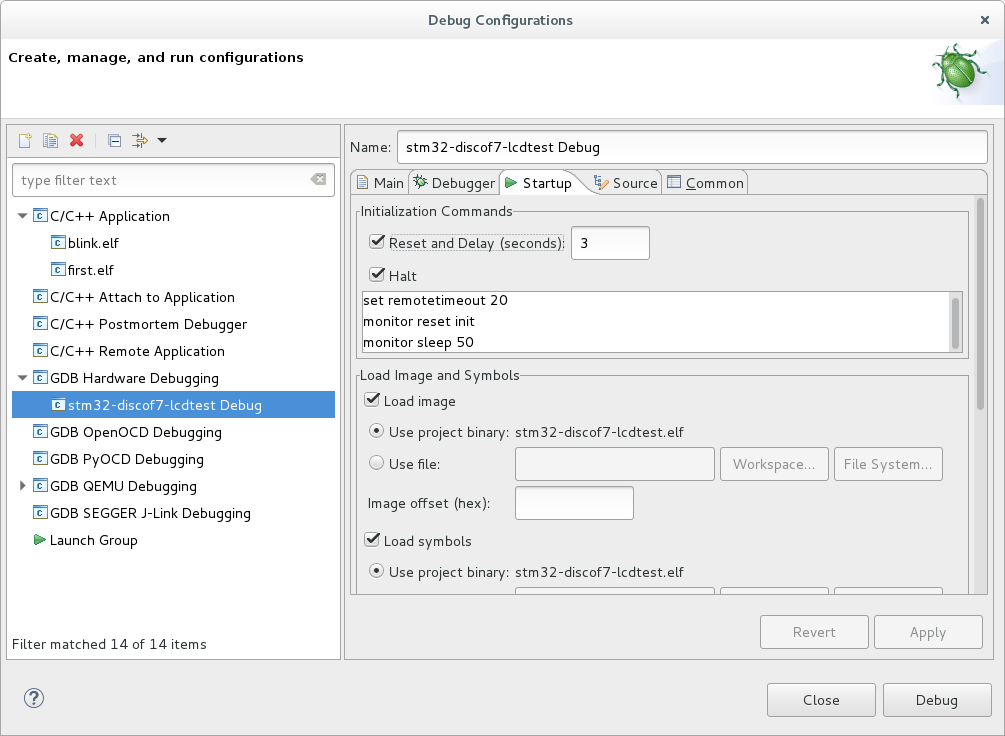
\includegraphics[width=12cm]{grafiken/debugger/GDBsetting3.png}
\label{ecplipse_GDB_setting3}
\caption{GDB Settings 'Startup'}
\end{center}
\end{figure}
Die Startup-Einstellungen müssen noch um die 'Initialization Commands' aus dem Bild \ref{ecplipse_GDB_setting3} ergänzt werden.
'Resume', 'Set breakpoint at: main', 'Load symbols', 'Load image' sind mit einem Haken versehen. 
\FloatBarrier
\subsection{Debuggen des ersten Projekts}
Um zu debuggen muss zuerst OpenOCD gestartet werden. Dazu muss einfach der Menüpunkt 'Run'>'External Tools'>'<Name der angelegten Konfiguration>' ausgewählt werden. Auf dem Target kann man anhand der blinkenden Status-LED feststellen, dass der Remote-Modus aktiviert wurde. Daraufhin muss der Debug-Button in Eclipse nur noch betätigt werden.
\subsection{Das erste Projekt war das letzte Projekt}
Als der Debugger bei der Projektarbeit ernsthaft benötigt wurde, setzte das Werkzeug plötzlich aus. Zuerst war es nicht mehr möglich das Projekt auf die Plattform zu befördern und schließlich war es nicht mehr möglich den Debugmodus auf der Hardware zu starten. 
Daraufhin wurde in einem Meeting des Teams besprochen es noch einmal mit einer anderen Installationsanleitung für den Debugger zu versuchen. Zuerst lieferte diese vielversprechende Ergebnisse, jedoch dann konnte auch hiermit keine Lösung herbeigeführt werden. 
Link zur alternativen Lösung: \url{http://www.carminenoviello.com/2015/01/07/setting-gcceclipse-toolchain-stm32nucleo-part-2/}